\documentclass[a4paper,11pt]{report}
\usepackage[utf8]{inputenc}
\usepackage[T1]{fontenc}
\usepackage[british]{babel}
\usepackage{geometry}
\usepackage{graphicx}
\usepackage{xcolor}
\usepackage{enumitem}
\usepackage{tabularx}
\usepackage{booktabs}
\usepackage{hyperref}
\usepackage{fancyhdr}
\usepackage{lastpage}
\usepackage{tikz}
\usepackage{tcolorbox}
\usepackage{fontawesome5}
\usepackage{multicol}

% Define DreamLab colours
\definecolor{dreamlabprimary}{RGB}{102, 51, 153}
\definecolor{dreamlabsecondary}{RGB}{255, 87, 34}
\definecolor{dreamlabaccent}{RGB}{0, 188, 212}
\definecolor{dreamlabdark}{RGB}{33, 33, 33}
\definecolor{dreamlablight}{RGB}{245, 245, 245}

% Page setup
\geometry{top=3cm, bottom=3cm, left=2.5cm, right=2.5cm}
\pagestyle{fancy}
\fancyhf{}
\fancyhead[L]{\textcolor{dreamlabprimary}{\textbf{DreamLab Brand Strategy}}}
\fancyhead[R]{\textcolor{dreamlabdark}{Page \thepage\ of \pageref{LastPage}}}
\fancyfoot[C]{\textcolor{dreamlabdark}{\small\textit{Confidential and Proprietary}}}
\renewcommand{\headrulewidth}{0.5pt}
\renewcommand{\footrulewidth}{0.3pt}

% Custom box style
\tcbset{
    dreambox/.style={
        colback=dreamlablight,
        colframe=dreamlabprimary,
        fonttitle=\bfseries,
        boxrule=2pt,
        arc=5mm,
        breakable
    }
}

\title{
    \vspace{-2cm}
    \textcolor{dreamlabprimary}{\Huge\bfseries DreamLab}\\[0.5cm]
    \textcolor{dreamlabdark}{\Large Brand Strategy Document}\\[0.3cm]
    \textcolor{dreamlabsecondary}{\large The Government-Endorsed Blueprint for Creative Technology}
}
\author{\textcolor{dreamlabdark}{Brand Strategy Team}}
\date{\textcolor{dreamlabdark}{\today}}

\begin{document}

\maketitle
\thispagestyle{empty}

\vspace{2cm}

\begin{tcolorbox}[dreambox, title=Executive Summary]
DreamLab positions itself as the North-West's premier creative technology agency, uniquely offering integrated AI, immersive experiences, and creative excellence at SME-accessible prices. As a ``government-endorsed blueprint'' for innovation, we bridge the gap between cutting-edge technology and practical business solutions, making enterprise-level capabilities available to ambitious businesses of all sizes.
\end{tcolorbox}

\tableofcontents
\newpage

\chapter{Brand Foundation}

\section{Brand Purpose}

\begin{tcolorbox}[dreambox, title=Our Why]
DreamLab exists to democratise access to transformative creative technology, empowering businesses across the North-West and beyond to compete on a global stage through innovation that's both accessible and sustainable.
\end{tcolorbox}

\subsection{Core Purpose Statement}
``Making the impossible accessible through creative technology that transforms businesses and communities.''

\subsection{Brand Belief}
We believe that every business, regardless of size, deserves access to the transformative power of AI, immersive experiences, and world-class creative direction. Innovation shouldn't be a luxury reserved for enterprises—it should be a tool for growth available to all ambitious organisations.

\section{Brand Vision \& Mission}

\begin{tcolorbox}[dreambox, title=Vision Statement]
To be recognised as the UK's leading integrated creative technology partner, setting the standard for how agencies combine AI, immersive experiences, and creative excellence to drive measurable business transformation.
\end{tcolorbox}

\begin{tcolorbox}[dreambox, title=Mission Statement]
We empower businesses to thrive in the digital age by seamlessly integrating cutting-edge AI, immersive technologies, and award-winning creative direction into accessible, results-driven solutions that deliver exceptional ROI.
\end{tcolorbox}

\chapter{Brand Positioning}

\section{Market Position}

\subsection{Positioning Statement}
For ambitious SMEs and forward-thinking enterprises in the North-West who need to harness the power of creative technology, DreamLab is the integrated agency that uniquely combines deep AI expertise, immersive technology capabilities, and award-winning creative direction at accessible price points. Unlike traditional agencies that specialise in single disciplines or enterprise consultancies with prohibitive costs, DreamLab delivers the full spectrum of creative technology services through our ``mesh fluency'' approach—seamlessly integrating all capabilities to create transformative solutions.

\subsection{Competitive Differentiation}

\begin{table}[h]
\centering
\begin{tabularx}{\textwidth}{X|X}
\toprule
\textbf{Traditional Agencies} & \textbf{DreamLab} \\
\midrule
Single discipline focus & Integrated multi-discipline expertise \\
High enterprise pricing & SME-accessible modular pricing \\
Technology OR creative & Technology AND creative excellence \\
Project-based relationships & Partnership-based growth model \\
Limited R\&D capabilities & University \& GMCA R\&D partnerships \\
Siloed service delivery & Mesh fluency across all capabilities \\
\bottomrule
\end{tabularx}
\end{table}

\section{Unique Value Propositions}

\begin{enumerate}
    \item \textbf{Government-Endorsed Innovation}: Recognised partnerships with GMCA and academic institutions position us as the trusted blueprint for creative technology innovation.
    
    \item \textbf{Mesh Fluency}: Our unique ability to seamlessly integrate AI, immersive tech, and creative excellence under one roof—no handoffs, no silos, just cohesive solutions.
    
    \item \textbf{Accessible Excellence}: Enterprise-level capabilities delivered through modular, scalable solutions that fit SME budgets and growth trajectories.
    
    \item \textbf{Measurable Impact}: Performance-based pricing models and clear KPIs ensure our success is directly tied to client outcomes.
    
    \item \textbf{Sustainable Innovation}: Focus on long-term partnerships and responsible technology deployment that considers environmental and social impact.
\end{enumerate}

\chapter{Brand Values}

\section{Core Values Framework}

\begin{tcolorbox}[dreambox, title=1. Innovation with Purpose]
\textbf{What it means}: We innovate not for innovation's sake, but to solve real business challenges and create tangible value.\\
\textbf{How we live it}: Every project begins with understanding the ``why'' before exploring the ``how'', ensuring technology serves strategic objectives.
\end{tcolorbox}

\begin{tcolorbox}[dreambox, title=2. Accessible Excellence]
\textbf{What it means}: World-class quality shouldn't be exclusive to enterprises. We make excellence achievable for all ambitious organisations.\\
\textbf{How we live it}: Modular pricing, transparent processes, and education-first approach to client relationships.
\end{tcolorbox}

\begin{tcolorbox}[dreambox, title=3. Collaborative Creativity]
\textbf{What it means}: The best solutions emerge from the intersection of diverse perspectives and disciplines.\\
\textbf{How we live it}: Cross-functional teams, client co-creation sessions, and active participation in the regional innovation ecosystem.
\end{tcolorbox}

\begin{tcolorbox}[dreambox, title=4. Sustainable Growth]
\textbf{What it means}: We build for the long term—for our clients, our team, and our community.\\
\textbf{How we live it}: Partnership-based client relationships, continuous learning culture, and commitment to regional economic development.
\end{tcolorbox}

\begin{tcolorbox}[dreambox, title=5. Transparent Impact]
\textbf{What it means}: Clear communication, measurable results, and honest partnerships drive everything we do.\\
\textbf{How we live it}: Regular reporting, open-book project management, and performance-based pricing models.
\end{tcolorbox}

\chapter{Brand Personality}

\section{Brand Archetype}

DreamLab embodies the \textbf{Magician} archetype with elements of the \textbf{Sage}:

\begin{itemize}
    \item \textbf{The Magician}: We transform the ordinary into the extraordinary, making the impossible possible through creative technology
    \item \textbf{The Sage}: We share knowledge openly, educate our clients, and act as trusted advisors in their digital transformation journey
\end{itemize}

\section{Personality Traits}

\subsection{Primary Traits}

\begin{multicols}{2}
\begin{itemize}
    \item \textbf{Innovative}: Constantly pushing boundaries
    \item \textbf{Approachable}: Accessible and down-to-earth
    \item \textbf{Expert}: Deep technical and creative mastery
    \item \textbf{Collaborative}: Partnership-focused
    \item \textbf{Ambitious}: Growth-oriented mindset
    \item \textbf{Pragmatic}: Results over rhetoric
\end{itemize}
\end{multicols}

\subsection{Brand Voice}

\begin{tcolorbox}[dreambox, title=Voice Characteristics]
\begin{itemize}
    \item \textbf{Confident but not arrogant}: We know our expertise but remain humble and helpful
    \item \textbf{Technical but accessible}: We translate complexity into clarity without dumbing down
    \item \textbf{Inspirational but practical}: We paint the vision while providing the roadmap
    \item \textbf{Professional but personable}: We maintain high standards while being genuinely friendly
\end{itemize}
\end{tcolorbox}

\section{Brand Tone Guidelines}

\begin{table}[h]
\centering
\begin{tabularx}{\textwidth}{X|X|X}
\toprule
\textbf{Context} & \textbf{Tone} & \textbf{Example} \\
\midrule
Sales conversations & Consultative, helpful & ``Let's explore how AI could streamline your operations...'' \\
Technical discussions & Clear, educational & ``RAG technology enables your data to...'' \\
Marketing content & Inspirational, accessible & ``Transform your business with technology that works as hard as you do'' \\
Client updates & Transparent, professional & ``This sprint delivered X, with Y impact on your KPIs'' \\
\bottomrule
\end{tabularx}
\end{table}

\chapter{Target Audiences}

\section{Primary Audience Segments}

\subsection{Ambitious SMEs}

\begin{tcolorbox}[dreambox, title=Profile]
\begin{itemize}
    \item Regional businesses with 10-250 employees
    \item Annual revenue £1M-£50M
    \item Growth-focused leadership
    \item Digital transformation readiness
    \item Located primarily in North-West England
\end{itemize}
\end{tcolorbox}

\textbf{Key Motivations}:
\begin{itemize}
    \item Competing with larger competitors
    \item Operational efficiency gains
    \item Customer experience enhancement
    \item Future-proofing their business
\end{itemize}

\textbf{Pain Points}:
\begin{itemize}
    \item Limited internal tech expertise
    \item Budget constraints for innovation
    \item Risk aversion to new technology
    \item Need for proven ROI
\end{itemize}

\subsection{Tech Startups \& Scale-ups}

\begin{tcolorbox}[dreambox, title=Profile]
\begin{itemize}
    \item Venture-backed or bootstrapped
    \item 5-50 employees
    \item Manchester/Liverpool tech hubs
    \item B2B or B2C digital products
    \item Rapid growth trajectory
\end{itemize}
\end{tcolorbox}

\textbf{Key Motivations}:
\begin{itemize}
    \item Speed to market
    \item Technical excellence
    \item Investor impressiveness
    \item User acquisition and retention
\end{itemize}

\subsection{Public Sector \& Cultural Institutions}

\begin{tcolorbox}[dreambox, title=Profile]
\begin{itemize}
    \item Local councils and NHS trusts
    \item Museums and cultural venues
    \item Educational institutions
    \item Tourism organisations
    \item Procurement-driven processes
\end{itemize}
\end{tcolorbox}

\textbf{Key Motivations}:
\begin{itemize}
    \item Public engagement
    \item Accessibility compliance
    \item Social value creation
    \item Budget efficiency
\end{itemize}

\section{Audience Personas}

\subsection{Primary Persona: Ambitious Anya}

\begin{tcolorbox}[dreambox]
\textbf{Demographics}: 28-40 years, Startup Founder/CTO, Manchester-based\\
\textbf{Psychographics}: Tech-savvy, risk-tolerant, network-driven, growth-obsessed\\
\textbf{Goals}: Scale rapidly, impress investors, build exceptional products\\
\textbf{Challenges}: Limited resources, time pressure, technical complexity\\
\textbf{How DreamLab Helps}: Rapid MVP development, AI integration, investor-ready demos
\end{tcolorbox}

\subsection{Secondary Persona: Established Ed}

\begin{tcolorbox}[dreambox]
\textbf{Demographics}: 45-60 years, SME Owner/MD, Regional manufacturing\\
\textbf{Psychographics}: Pragmatic, ROI-focused, relationship-driven, cautiously innovative\\
\textbf{Goals}: Modernise operations, increase efficiency, stay competitive\\
\textbf{Challenges}: Legacy systems, change management, budget justification\\
\textbf{How DreamLab Helps}: Phased digital transformation, clear ROI metrics, ongoing support
\end{tcolorbox}

\chapter{Brand Architecture}

\section{Service Brand Framework}

\subsection{Core Service Pillars}

\begin{figure}[h]
\centering
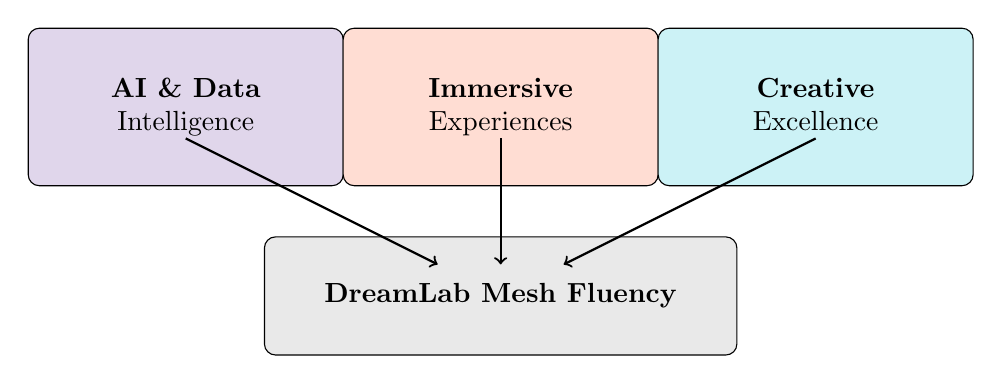
\begin{tikzpicture}[scale=0.8]
    % AI & Data pillar
    \node[draw, fill=dreamlabprimary!20, rounded corners, minimum width=4cm, minimum height=2cm] at (0,0) {
        \begin{tabular}{c}
        \textbf{AI \& Data}\\
        Intelligence
        \end{tabular}
    };
    
    % Immersive pillar
    \node[draw, fill=dreamlabsecondary!20, rounded corners, minimum width=4cm, minimum height=2cm] at (5,0) {
        \begin{tabular}{c}
        \textbf{Immersive}\\
        Experiences
        \end{tabular}
    };
    
    % Creative pillar
    \node[draw, fill=dreamlabaccent!20, rounded corners, minimum width=4cm, minimum height=2cm] at (10,0) {
        \begin{tabular}{c}
        \textbf{Creative}\\
        Excellence
        \end{tabular}
    };
    
    % DreamLab at the center
    \node[draw, fill=dreamlabdark!10, rounded corners, minimum width=6cm, minimum height=1.5cm] at (5,-3) {
        \textbf{DreamLab Mesh Fluency}
    };
    
    % Connecting lines
    \draw[thick, ->] (0,-0.5) -- (4,-2.5);
    \draw[thick, ->] (5,-0.5) -- (5,-2.5);
    \draw[thick, ->] (10,-0.5) -- (6,-2.5);
\end{tikzpicture}
\caption{DreamLab Service Integration Model}
\end{figure}

\subsection{Service Sub-brands}

\begin{enumerate}
    \item \textbf{DreamLab Intelligence}: AI/ML solutions, data analytics, automation
    \item \textbf{DreamLab Immersive}: VR/AR experiences, virtual production, spatial computing
    \item \textbf{DreamLab Creative}: Brand design, content creation, campaign development
    \item \textbf{DreamLab Labs}: R\&D partnerships, innovation workshops, prototyping
    \item \textbf{DreamLab Growth}: Business advisory, funding support, scaling strategies
\end{enumerate}

\section{Partnership Brands}

\begin{itemize}
    \item \textbf{DreamLab Education}: Training programmes and workshops
    \item \textbf{DreamLab Ventures}: Startup incubation and acceleration (future)
    \item \textbf{DreamLab Foundation}: Social impact and community initiatives (future)
\end{itemize}

\chapter{Visual Identity Guidelines}

\section{Logo and Mark}

\begin{tcolorbox}[dreambox, title=Logo Description]
The DreamLab logo combines technological precision with creative fluidity:
\begin{itemize}
    \item Primary mark: Interconnected nodes forming a constellation pattern
    \item Represents our ``mesh fluency'' and integrated approach
    \item Dynamic gradient from primary purple to secondary orange
    \item Clean, modern typography with subtle tech-inspired details
\end{itemize}
\end{tcolorbox}

\textit{[Placeholder for logo variations and usage guidelines]}

\section{Colour Palette}

\subsection{Primary Colours}

\begin{table}[h]
\centering
\begin{tabularx}{\textwidth}{X|c|c|c}
\toprule
\textbf{Colour} & \textbf{Hex} & \textbf{RGB} & \textbf{Usage} \\
\midrule
DreamLab Purple & \#6633CC & 102, 51, 153 & Primary brand colour, headers \\
DreamLab Orange & \#FF5722 & 255, 87, 34 & Accent, CTAs, energy \\
DreamLab Cyan & \#00BCD4 & 0, 188, 212 & Digital, innovation \\
DreamLab Dark & \#212121 & 33, 33, 33 & Text, professional \\
DreamLab Light & \#F5F5F5 & 245, 245, 245 & Backgrounds, space \\
\bottomrule
\end{tabularx}
\end{table}

\subsection{Secondary Palette}

\textit{[Placeholder for extended colour palette with tints and shades]}

\section{Typography}

\subsection{Primary Typefaces}

\begin{tcolorbox}[dreambox, title=Typography System]
\textbf{Headlines}: Montserrat Bold/Black
\begin{itemize}
    \item Modern, geometric sans-serif
    \item Conveys strength and innovation
    \item Used for impact and hierarchy
\end{itemize}

\textbf{Body Text}: Inter Regular/Medium
\begin{itemize}
    \item Highly legible screen font
    \item Professional and approachable
    \item Optimised for digital reading
\end{itemize}

\textbf{Technical/Code}: JetBrains Mono
\begin{itemize}
    \item Monospaced for technical content
    \item Reinforces our technical expertise
    \item Used sparingly for emphasis
\end{itemize}
\end{tcolorbox}

\section{Visual Elements}

\subsection{Graphic Devices}

\begin{enumerate}
    \item \textbf{Mesh Patterns}: Interconnected node networks representing integration
    \item \textbf{Gradient Overlays}: Smooth transitions between brand colours
    \item \textbf{Data Visualisations}: Clean, modern charts and infographics
    \item \textbf{Abstract Tech Elements}: Circuit patterns, particle effects, geometric shapes
\end{enumerate}

\subsection{Photography Style}

\begin{tcolorbox}[dreambox, title=Photography Guidelines]
\begin{itemize}
    \item \textbf{People}: Authentic, diverse, engaged in creative/tech work
    \item \textbf{Technology}: Clean, modern, with dramatic lighting
    \item \textbf{Environments}: Modern workspaces, North-West landmarks
    \item \textbf{Abstract}: Conceptual imagery for innovation themes
\end{itemize}

Treatment: High contrast, selective colour highlighting, subtle tech overlays
\end{tcolorbox}

\subsection{Iconography}

\textit{[Placeholder for icon style guide and examples]}

\chapter{Brand Application}

\section{Digital Touchpoints}

\subsection{Website}
\begin{itemize}
    \item Hero section with dynamic mesh animation
    \item Case study carousel showcasing integrated projects
    \item Interactive service explorer
    \item Client portal for project management
    \item Resource hub with guides and insights
\end{itemize}

\subsection{Social Media}
\begin{itemize}
    \item LinkedIn: Thought leadership and case studies
    \item Instagram: Behind-the-scenes creative process
    \item Twitter/X: Industry insights and quick updates
    \item YouTube: Demo reels and educational content
\end{itemize}

\section{Physical Touchpoints}

\subsection{Office Environment}
\begin{itemize}
    \item Reception: Large mesh pattern installation
    \item Meeting rooms: Named after innovation themes
    \item Demo spaces: Immersive technology showcases
    \item Collaboration areas: Branded with values
\end{itemize}

\subsection{Events and Exhibitions}
\begin{itemize}
    \item Modular exhibition stands reflecting service integration
    \item Interactive demos at Digital City Festival
    \item Branded workshop materials
    \item Speaker presentation templates
\end{itemize}

\section{Marketing Collateral}

\subsection{Print Materials}
\begin{itemize}
    \item Business cards with spot UV mesh pattern
    \item Capabilities brochure with AR triggers
    \item Proposal templates with dynamic layouts
    \item Leave-behind cards for each service pillar
\end{itemize}

\subsection{Digital Materials}
\begin{itemize}
    \item Email signature system
    \item PowerPoint/Keynote templates
    \item Digital brochures and one-pagers
    \item Animated service explainers
\end{itemize}

\chapter{Brand Governance}

\section{Brand Management Structure}

\subsection{Brand Champions}
\begin{itemize}
    \item \textbf{Brand Guardian}: CMO/Marketing Director
    \item \textbf{Creative Director}: Visual consistency
    \item \textbf{Content Lead}: Voice and messaging
    \item \textbf{Project Managers}: Client-facing consistency
\end{itemize}

\subsection{Approval Process}
\begin{enumerate}
    \item All external communications reviewed by brand team
    \item Major campaigns approved by leadership
    \item Partner co-branding requires brand guardian sign-off
    \item Quarterly brand audits to ensure consistency
\end{enumerate}

\section{Brand Guidelines Distribution}

\begin{itemize}
    \item Digital brand portal for all team members
    \item Condensed guidelines for partners
    \item Client co-branding toolkit
    \item Vendor/supplier brand standards
\end{itemize}

\section{Evolution and Flexibility}

\begin{tcolorbox}[dreambox, title=Living Brand Principle]
While maintaining core consistency, the DreamLab brand is designed to evolve with technology and market needs. Annual reviews will assess:
\begin{itemize}
    \item Market positioning effectiveness
    \item Visual identity relevance
    \item Message resonance with audiences
    \item Competitive differentiation
\end{itemize}
\end{tcolorbox}

\chapter{Implementation Roadmap}

\section{Phase 1: Foundation (Months 1-3)}
\begin{itemize}
    \item Finalise visual identity system
    \item Develop core marketing materials
    \item Train team on brand guidelines
    \item Launch internal brand portal
\end{itemize}

\section{Phase 2: Launch (Month 4)}
\begin{itemize}
    \item Unveil brand at Digital City Festival
    \item Deploy new website and digital presence
    \item PR campaign announcing positioning
    \item Client communication of rebrand
\end{itemize}

\section{Phase 3: Amplification (Months 5-8)}
\begin{itemize}
    \item Content marketing campaign
    \item Thought leadership programme
    \item Strategic partnership announcements
    \item Award submissions
\end{itemize}

\section{Phase 4: Evolution (Months 9-12)}
\begin{itemize}
    \item Brand perception research
    \item Refinement based on feedback
    \item Expansion of brand applications
    \item Annual brand review
\end{itemize}

\appendix

\chapter{Brand Glossary}

\begin{description}
    \item[Mesh Fluency] Our unique ability to seamlessly integrate multiple disciplines
    \item[Creative Technology] The intersection of artistic vision and technical innovation
    \item[Accessible Excellence] Enterprise-quality solutions at SME-friendly prices
    \item[Government-Endorsed Blueprint] Recognition from GMCA and public sector as innovation standard
    \item[Sustainable Innovation] Technology deployment considering long-term impact
\end{description}

\chapter{Quick Reference}

\section{Elevator Pitch}
``DreamLab is the North-West's only creative technology agency that seamlessly integrates AI, immersive experiences, and award-winning creative direction—all at prices that make sense for ambitious SMEs. We're the government-endorsed blueprint for how businesses should approach digital transformation.''

\section{Key Messages}
\begin{enumerate}
    \item Integrated expertise across AI, immersive, and creative
    \item SME-accessible pricing for enterprise-level capabilities
    \item Proven partnerships with GMCA and universities
    \item Measurable ROI through performance-based models
    \item Local presence with global standards
\end{enumerate}

\section{Boilerplate}
DreamLab is Salford's premier creative technology agency, offering integrated AI, immersive experiences, and creative excellence to businesses across the North-West. With a team of 30 specialists and partnerships with leading universities and GMCA innovation hubs, DreamLab makes enterprise-level creative technology accessible to organisations of all sizes. Our unique ``mesh fluency'' approach ensures seamless integration across all digital disciplines, delivering transformative solutions that drive measurable business growth.

\end{document}